%%%%%%%%%%%%%%%%%%%%%%%%%%%%%%%%%%%%%%%%%%%%%%%%%%%%%%%%%%
%
% Vzor pro sazbu kvalifikační práce
%
% Západočeská univerzita v Plzni
% Fakulta aplikovaných věd
% Katedra informatiky a výpočetní techniky
%
% Petr Lobaz, lobaz@kiv.zcu.cz, 2016/03/14
%
%%%%%%%%%%%%%%%%%%%%%%%%%%%%%%%%%%%%%%%%%%%%%%%%%%%%%%%%%%

% Možné jazyky práce: czech, english
% Možné typy práce: BP (bakalářská), DP (diplomová)
\documentclass[czech,P5]{thesiskiv}

% Definujte údaje pro vstupní strany
%
% Jméno a příjmení; kvůli textu prohlášení určete, 
% zda jde o mužské, nebo ženské jméno.
\author{Petr Holický}
\declarationmale

%alternativa: 
%\declarationfemale

% Název práce
\title{Semestrální práce}

% Na titulní stranu a do textu prohlášení se automaticky vkládá 
% aktuální rok, resp. datum. Můžete je změnit:
%\titlepageyear{2016}
%\declarationdate{1. března 2016}

% Ve zvláštních případech je možné ovlivnit i ostatní texty:
%
%\university{Západočeská univerzita v Plzni}
%\faculty{Fakulta aplikovaných věd}
%\department{Katedra informatiky a výpočetní techniky}
%\subject{Bakalářská práce}
%\titlepagetown{Plzeň}
%\declarationtown{Plzni}

%%%%%%%%%%%%%%%%%%%%%%%%%%%%%%%%%%%%%%%%%%%%%%%%%%%%%%%%%%
%
% DODATEČNÉ BALÍČKY PRO SAZBU
% Jejich užívání či neužívání záleží na libovůli autora 
% práce
%
%%%%%%%%%%%%%%%%%%%%%%%%%%%%%%%%%%%%%%%%%%%%%%%%%%%%%%%%%%

% Zařadit literaturu do obsahu
\usepackage[nottoc,notlot,notlof]{tocbibind}

% code
\usepackage{listings}

% Umožňuje vkládání obrázků
\usepackage[pdftex]{graphicx}
\usepackage{float}

% Odkazy v PDF jsou aktivní; navíc se automaticky vkládá
% balíček 'url', který umožňuje např. dělení slov
% uvnitř URL
\usepackage[pdftex]{hyperref}
\hypersetup{colorlinks=true,
  unicode=true,
  linkcolor=black,
  citecolor=black,
  urlcolor=black,
  bookmarksopen=true}

% Při používání citačního stylu csplainnatkiv
% (odvozen z csplainnat, http://repo.or.cz/w/csplainnat.git)
% lze snadno modifikovat vzhled citací v textu
\usepackage[numbers,sort&compress]{natbib}

%práce s textem
\usepackage{amsmath}

%%%%%%%%%%%%%%%%%%%%%%%%%%%%%%%%%%%%%%%%%%%%%%%%%%%%%%%%%%
%
% VLASTNÍ TEXT PRÁCE
%
%%%%%%%%%%%%%%%%%%%%%%%%%%%%%%%%%%%%%%%%%%%%%%%%%%%%%%%%%%
\begin{document}
%
\maketitle
\tableofcontents


%%%%%%%%%%%%%%%%%%%%%%%%%%              ZADÁNÍ		 %%%%%%%%%%%%%%%%%%%%
\chapter{Zadání}
\textbf{Target}
\\\\
The main objective of the project is to develop a web application allowing tracking of \textbf{allocations/jobs/project assignments (this is SINGLE thing, pick whichever name you want)} of the department members. 
\\\\
Department employees participate in many different projects, with different size of allocation (x-hours per week) throughout time. The application is supposed to provide project managers with tooling to oversee their team members allocations (current and planned), ensure the person’s total allocation does not exceed 1.0 at any given moment, etc. 
\\\\
The most successful project implementation will be taken into use by the Department of Computer Science. 
\\\\
{\LARGE \textbf{Base Requirements [30p]}}
\\\\
\textbf{Roles}
\\\\
The application users take on several distinct roles, each with its own set of permissions and access to different functionalities. The roles may be combined. The following is the mapping between the roles and permissions. The role names are placeholders and may be changed by the developer to a degree. 
\begin{itemize}
             \item Unauthorized user 
             \begin{itemize}
             	\item Sign in 
             \end{itemize}
             \item  Regular authorized user
               \begin{itemize}
             	\item Review their own allocations/jobs/project assignments 
             	\item Log out 
             \end{itemize}
             \item Superior
             \begin{itemize}
             	\item Review the allocations/jobs/project assignments of all their subordinates 
             \end{itemize}
             \item Project manager 
               \begin{itemize}
             	\item Review the allocations/jobs/project assignments of all people (only) on their projects 
             	\item Input/edit allocations/jobs/project assignments of people on their projects 
             	\item See the aggregate workload of people they want to add to their project across all projects 
	             	\begin{itemize}
	             		\item  i.e., they see the sum of people’s allocations across projects, but do not see on which projects they are, nor the division of their allocations among projects 
	             		\item The aggregate is for 1) active assignments, 2) all assignments 
	             	\end{itemize}
             	\item Edit their projects’ information 
             \end{itemize}
             \item Department manager 
              \begin{itemize}
             	\item Same as project manager, but for all projects 
             \end{itemize}
              \item Secretariat
               \begin{itemize}
             	\item Register users 
             	\item Create projects 
             	\item Assign people to projects 
             	\item Edit projects and people information
             	\item Adds subordinates to superiors 
             \end{itemize}
\end{itemize}
Data hierarchy between roles goes in the following fashion: 
\\\\
Superior -> Worker (M:N) - relationship between workers in departmental hierarchy (independent on projects) 
\\\\
Project manager -> Project (M:1) - single person can have project manager role for multiple projects, but it has to be explicitly configured per-case 
\\\\
\textbf{User registration}
\\\\
Done primarily by the Secretariat role by inputting their Orion username into a proper form field. The application will hold the following user information: 
\begin{itemize}
             \item Full name 
             \item Orion login/username 
             \item Primary workplace 
             \item Email address 
\end{itemize}
Other user information is above the minimal project criteria. 
\\\\
\textbf{Login}
\\\\
A user logs in through orion username and generated password. Password is shown to registrator (Secretariat) upon registration and must be changed by user upon first login. \textbf{This requirement can be replaced by Kerberos integration (see Optional Functional Requirements below)}
\\\\
\textbf{Project}
\\\\
The project contains (at least) the following data: 
\begin{itemize}
             \item Project name 
             \item Project manager (orion login) 
             \item Timespan (from-to; end date is optional, if not entered viewed as indefinite) 
             \item Description/Note 
\end{itemize}
\textbf{Allocation/job/project assignment}
\\\\
The creation of the allocation/job/project assignment contains the following data: 
\begin{itemize}
             \item Worker
             \item Project
             \item Allocation scope (as a ratio of FTE) 
             \begin{itemize}
	             \item FTE=full time equivalent=40h/week 
	             \item Entered and displayed in hours/week or x/1FTE  
             \end{itemize}
             \item Timespan (from-to) 
             \item Description/Note 
\end{itemize}
The allocation/job/project assignment has a lifecycle with the following distinct states which need to be recognizable in the application (the names are not compulsory): 
\begin{itemize}
             \item Inactive
             \begin{itemize}
	             \item Draft/intended 
	             \item Cancelled/unrealized 
	              \item Past
             \end{itemize}
             \item Active
\end{itemize}
Some transitions between these states can be calculated or automatically triggered (unrealized, past), while others need to be triggered by the users with proper permissions (active, cancelled). 
\\\\
\textbf{Extra-functional requirements}
\\\\
GUI will be primarily in CZ (does not apply to Erasmus students). 
\\\\
{\LARGE \textbf{Optional functional requirements}}
\\\\
{\large \textbf{User Registration and authentication}}
\begin{itemize}
             \item User data import from UWB information systems (STAG integration) based on orion login [+8p] 
  		\\ https://is-stag.zcu.cz/napoveda/web-services/ws\_changelists.html 
             \item Integration with UWB single-sign-on system (SAML, Kerberos) [+5p] (replaces default username and password authentication) 
   		\\ https://support.zcu.cz/index.php/Kerberos 
\end{itemize}
{\large \textbf{Notifications}}
\begin{itemize}
             \item Application will send notifications via email triggered by appropriate events to the proper users. [+4b] 
   		\\ Minimum list of events:
   	  \begin{itemize}
	             \item activation of a project/assignment, 
	             \item  expiration of assignment in near future 
	              \item project creation and assignment 
             \end{itemize}
\end{itemize}
{\large \textbf{UX}}
\begin{itemize}
             \item Whenever multiple allocations/jobs/project assignments are displayed, the list can be filtered, sorted, grouped, and appropriate aggregation functions (e.g., sums) will be displayed. [+3p] 
             \item When planning project/person’s assignments a user-friendly display of their existing allocations over time with sliding time window or similar feature (like, for example, an online calendar). [+5p] 
             \item charts/graphs where appropriate [+3p]
             \item The ability to enter and view assignments scopes in both x/1FTE and hours/week. [+1p] 
             \item Bilingual, CZ/EN GUI, or at least an infrastructure prepared for it. [+3p for infrastructure, +1p for translations] 
\end{itemize}
{\large \textbf{Deployment and maintenance}}
\begin{itemize}
             \item Detailed maintenance guide [+2p] for installation and standard/regular maintenance task 
             \item Detailed user guide [+2p] with screenshots for the main use-cases 
\end{itemize}
{\large \textbf{Other}}
\begin{itemize}
             \item SPA + WS API architecture [+10p] 
             \item customizable notification settings (which notifications user wants to receive) [+4p] 
             \item exports (ask ppicha@kiv.zcu.cz for details on what to export)  
             \begin{itemize}
	             \item to CSV [+2p] 
	             \item PDF (pretty, not just plain text!) [+4p] 
             \end{itemize}
\end{itemize}
{\large \textbf{General Requirements}}
\\\\
\textbf{Allowed technology} \\
Java \\
C\# \\
 Ruby \\
Python \\
Node.js (Typescript is mandatory) \\
PHP (Laravel or Symphony or Nette is mandatory)
\newpage
\textbf{Implementation requirements }
\begin{itemize}
             \item Correct implementation of selected architecture 
             \item Reasonably long methods (typically 50-100 lines, exceptions allowed) 
             \item Well-commented methods/functions, data models, attributes 
             \item User management module covered with automated tests (unit, integration) 
             \item Configurations must be read from property files, env variables, etc. 
\end{itemize}
 
%%%%%%%%%%%%%%%%%%%%%%%%%%            ANALYTICKÁ ČÁST          %%%%%%%%%%%%%%%%%% %%%%%%%%%%%%%%%%%%%%%%%%
%	NO	%
%%%%%%%%%%%%%%%%%%%%%%%%%%            REALIZAČNÍ ČÁST           %%%%%%%%%%%%%%%%%% %%%%%%%%%%%%%%%%%%%%%%%%
\chapter{Implementace}
Základ aplikace vychází z projetku který byl vytvořen na cvičení.
\\\\
\textbf{Využité technologie:}
\begin{itemize}
             \item Spring Framework
             \item Thymeleaf
             \item Tomcat
             \item Docker (MySQL)
             \item Mockito
\end{itemize}
\textbf{Struktura projektu:}
\begin{itemize}
             \item Core
             \item Jdbc
             \item Web
\end{itemize}
\textbf{Implementovaná rozšíření:}
\begin{itemize}
             \item Infrastruktura pro více jazyků
             \item Uživatelská příručka s obrázky
             \item Zobrazení úvazku v hodinách a poměru FTE
\end{itemize}
\section{Core}
Tento modul pracuje s daty. Dělí se na 3 hlavní sekce:
\begin{itemize}
             \item Domain
             \item Repository
             \item Service
\end{itemize}
\subsection{Domain}
Zde jsou definovány všechny základní třídy:
\begin{itemize}
             \item Assignment
             \item Project
             \item Subordinate
             \item User
\end{itemize}
Třída User představuje uživatele pracující s aplikací. Tito uživatelé mohou obsahovat podřízené, což je realizovano přes třídu Subordinate. Třída Project definuje projekty do kterých jsou uživatelé přidáni. Jejich přidání do projektu, a tedy i následná definice přiřazení, je popáno pomocí třídy Assignment.
\subsection{Repository}
Zde jsou definovány rozhraní, přes která se ukládají a načítají data typu \texttt{Domain}. Tyto rozhraní jsou zde navíc implementována do tříd, které jsou schopné data ukládat do paměti.
\subsection{Service}
Tato sekce obsahuje \texttt{Service} třídy, které definují jaké akce lze provádět nad \texttt{Domain} daty. Tyto třídy zpravidla využívají \texttt{Repository} rozhraní k provedení požadované akce.
\section{Jdbc}
Tento modul slouží jako prostředek pro komunikaci s databází. Dělí se na 2 sekce:
\begin{itemize}
             \item Mapper
             \item Repository
\end{itemize}
\subsection{Mapper}
Tato sekce obsahuje mapper pro každou třídu z \texttt{Domain}. Tyto třídy ukládají nahraná data z databáze, která se poté zobrazí uživateli.
\subsection{Repository}
Stejně jako v předešlém modulu \texttt{Core}, zde třídy slouží k ukládání a načítání dat. Tentokrát se ale pracuje s daty přímo z databáze. Tedy tyto třídy obsahují seškeré SQL příkazy potřebné pro komunikaci aplikace s databází.
\section{Web}
Tento modul slouží jako vstupní bod aplikace a je zodpovědný za komunikaci s uživatelem. Tedy zpracování požadavků a vykreslování samotného webu. Děli se na 4 hlavní sekce:
\begin{itemize}
             \item Webapp
             \item Controller
             \item VO
             \item Resources
\end{itemize}
\subsection{Webapp}
Slouží ke spuštení samotné aplikace. Je zde definován celkový kontext a nastavení aplikace. Také obsahuje potřebné třídy pro realizaci více lokalizací aplikace.
\subsection{Controller}
Zde třídy definují url adresy aplikace a jak se aplikace zachová na požadavky od uživatele. Tedy pokud uživatel zažádá o html stránku přes validní url adresu, tak načte potřebná data a stránku vykreslí. Aplikace využívá server-side rendering. Jestliže přijde požadavek na zpracování akce od uživatale, např.: stisknutí tlačítka, tak také definuje jak se aplikace zachová. Po zpracování požadavku předá/vyvolá příslušnou metodu ze \texttt{Service} tříd z modulu \texttt{Core}, která požadavek zpracuje už interně.
\subsection{VO}
Zkratka pro \texttt{Value Object}. Slouží k uchování dat než dojde k jejich zpracování. Využito především ve formulářích, které uživatelé vyplňují.
\subsection{Resources}
Obsahuje pořebné soubory pro iniciální spuštění s databází, veškeré html soubory a \texttt{properties} soubory pro angličtinu a češtinu.

%%%%%%%%%%%%%%%%%%%%%%%%%%            UŽVATELSKÁ PŘÍRUČKA        %%%%%%%%%%%%%%%%%%%%%%%% %%%%%%%%%%%%%%%%%
\chapter{Uživatelská příručka}
\section{Přihlášení}
Výchozí bod aplikace je \texttt{/pia-sp/spring/}, tedy v našem případě:
\\\\
\texttt{http://localhost:8080/pia-sp/spring/}
\\\\
Jelikož nejsme přihlášení, tak budeme automaticky přesměrováni na přihlašovací stránku \texttt{/pia-sp/spring/login} \ref{fig:login}.
\begin{figure}[h]
	\centering
	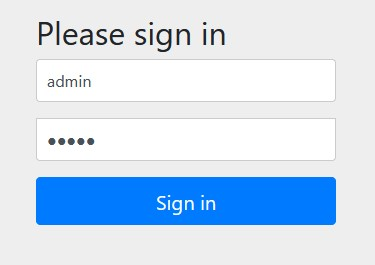
\includegraphics[width=0.45\textwidth]{Images/login.jpg}
	\caption{Přihlašovací stránka}
	\label{fig:login} 
\end{figure}
\\
Po úspěšném přihlášení můžeme vstoupit do aplikace, neboli jsme přesměrováni zpět na původní zadanou adresu, tedy v našem případě \texttt{/pia-sp/spring/} \ref{fig:index}.
\\\\
Výchozí uživatelé jsou:
\begin{itemize}
             \item admin
             \item dmanager
             \item pmanager
             \item superior
             \item default
             \item default2
\end{itemize}
Heslo uživatele admin je \textit{admin}. Pro ostatní uživatele je heslo \textit{password}. Uživatel admin má práva sekretariátu, ostatní uživatelé odpovídají dalším právům následovně: department manager, project manager, superior a běžný uživatel.

\section{Ůvodní stránka}
Ůvodní stránka aplikace. Její obsah se liší podle role přihlášeného uživatele.
\begin{figure}[H]
	\centering
	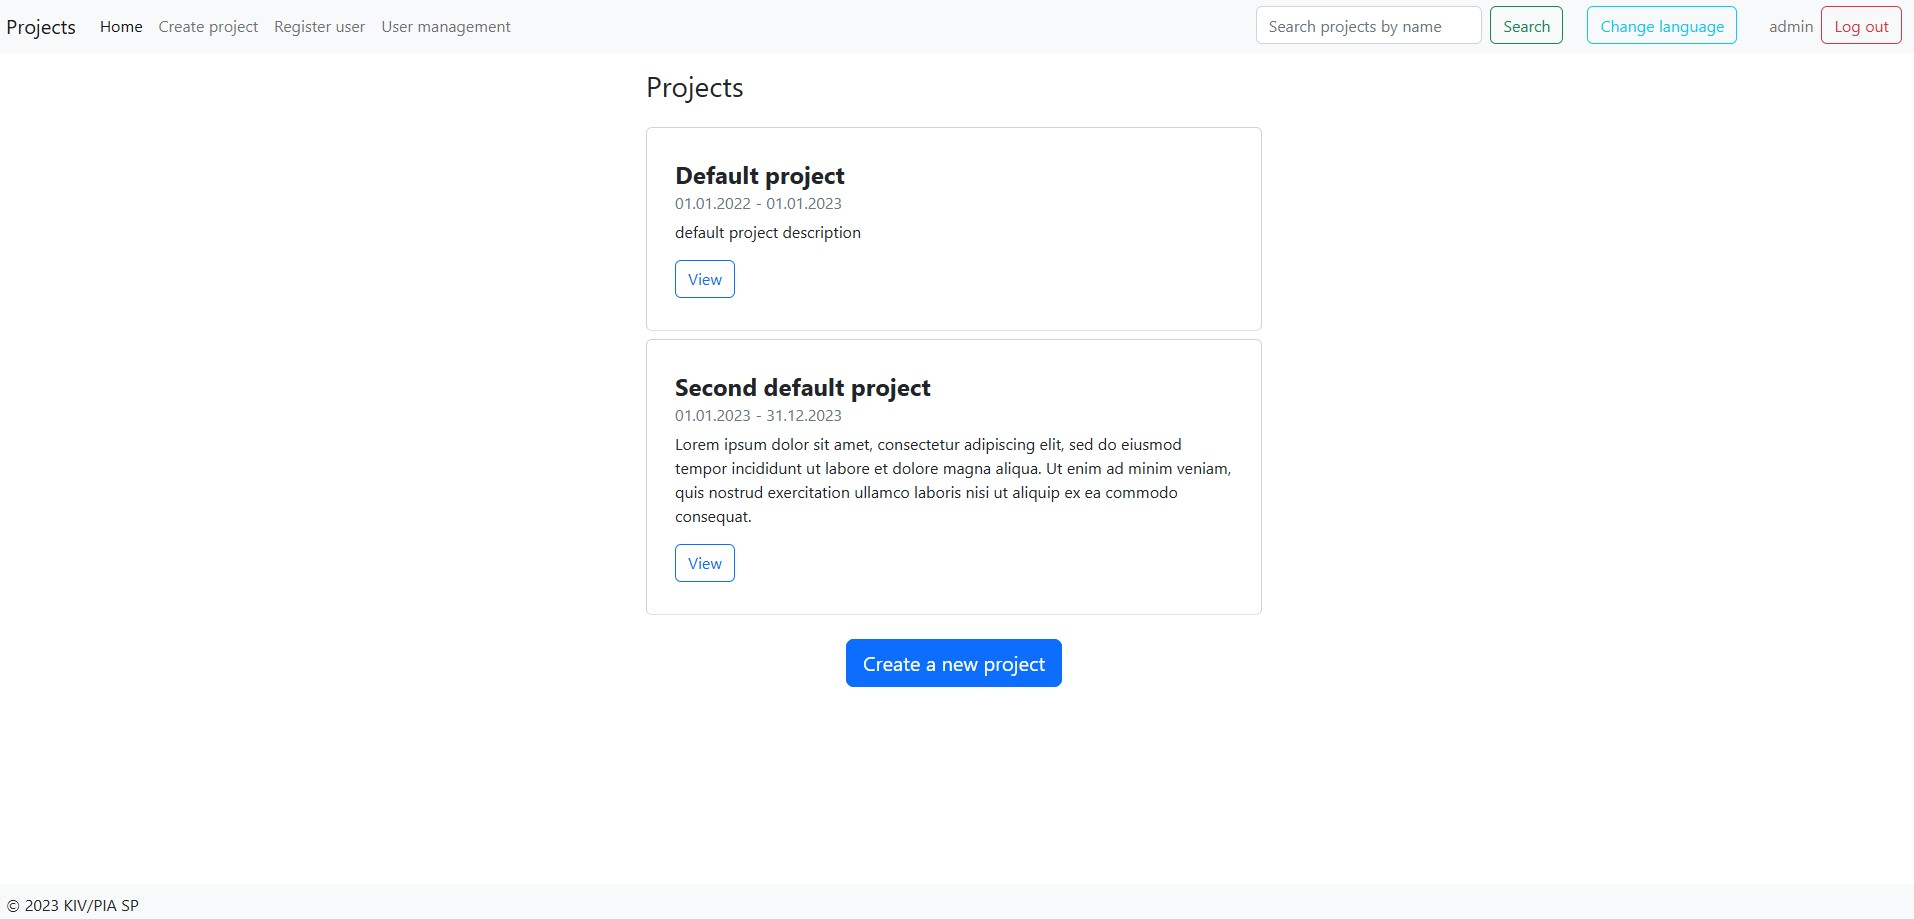
\includegraphics[width=\textwidth]{Images/index.jpg}
	\caption{Ůvodní stránka pro sekretariát}
	\label{fig:index} 
\end{figure}
Položky v menu jako \texttt{Register user} a \texttt{Create project} vidí pouze sekretariát. Sekretariát a Department manager si také mohou zobrazit všechny projekty naopak od Projekt manažera, který si může zobrazit jen svoje projekty \ref{fig:indexpmanager}, či od běžného uživatele.
\begin{figure}[H]
	\centering
	\includegraphics[width=0.65\textwidth]{Images/index\_pmanager.jpg}
	\caption{Zobrazení projektů pro Projekt manažera}
	\label{fig:indexpmanager} 
\end{figure}

\section{Registrace uživatele}
Stránka obsahující formulář pro registraci uživatele \ref{fig:reg}.
\begin{figure}[H]
	\centering
	\includegraphics[width=\textwidth]{Images/register\_user.jpg}
	\caption{Vytvoření nového uživatele}
	\label{fig:reg} 
\end{figure}
\newpage
 Pokud uživatel již existuje \ref{fig:regfail} nebo nejsou vyplněna všechna pole formuláře, tak uživatel o tom bude informován.
 \begin{figure}[H]
	\centering
	\includegraphics[width=\textwidth]{Images/register\_user\_fail.jpg}
	\caption{Uživatel již existuje}
	\label{fig:regfail} 
\end{figure}
\newpage

\section{Vytvoření nového projektu}
Stránka obsahující formulář pro vytvoření nového projektu \ref{fig:createproject}. Formulář opět kontroluje zda projekt již existuje, všechna pole jsou vyplněna a že zadaný rozestup pro datum je validní.
 \begin{figure}[H]
	\centering
	\includegraphics[width=\textwidth]{Images/create\_project.jpg}
	\caption{Vytvoření nového projektu}
	\label{fig:createproject} 
\end{figure}
\newpage

\section{Podrobné zobrazení projektu}
Stránka zobrazující detaily projektu. Jsou zde vidět přiřazení uživatelé a detaily o jejich přiřazení \ref{fig:viewProjectSec}. Podle role přihlášeného uživatele lze upravit projek či přiřazení uživatele \ref{fig:viewProjectMan}, nebo přidat nového uživatele do projektu \ref{fig:viewProjectAdd}. 
 \begin{figure}[H]
	\centering
	\includegraphics[width=\textwidth]{Images/project\_view\_secretariat.jpg}
	\caption{Zobrazení projektu pro Sekretariát}
	\label{fig:viewProjectSec} 
\end{figure}
 \begin{figure}[H]
	\centering
	\includegraphics[width=\textwidth]{Images/project\_view\_secretariat\_assign\_user.jpg}
	\caption{Přidání uživatele do projektu}
	\label{fig:viewProjectAdd} 
\end{figure}
 \begin{figure}[H]
	\centering
	\includegraphics[width=\textwidth]{Images/project\_view\_manager.jpg}
	\caption{Zobrazení projektu pro manažery}
	\label{fig:viewProjectMan} 
\end{figure}

\section{Úprava projektu a přiřazených uživatelů}
Ze stránky projektu lze upravit projekt \ref{fig:editProject} nebo přiřazení uživatele \ref{fig:editAssignment}. Oba formůláře jsou opět ošetřeny na validní vstupy.  
 \begin{figure}[H]
	\centering
	\includegraphics[width=\textwidth]{Images/edit\_project.jpg}
	\caption{Upravení projektu}
	\label{fig:editProject} 
\end{figure}
 \begin{figure}[H]
	\centering
	\includegraphics[width=\textwidth]{Images/edit\_assignment.jpg}
	\caption{Upravení přiřazení uživatele}
	\label{fig:editAssignment} 
\end{figure}
\newpage

\section{Správa uživatelů}
Tato stránka se liší nejvíce podle role přihlášeného uživatele. Podle přihlášené role vidí uživatel jiná data v tabulce. Každý záznam v tabulce je interaktivní, kde po kliknutí se objeví nová řada obsahující projekty spojené s tímto uživatelem a jeho přiřazení do těchto projektů.
\begin{itemize}
             \item \textbf{Sekretariát:} vidí všechny uživatele a jejich jednotlivá přiřazení \ref{fig:userManSec}. Uživatele tady lze může i upravit \ref{fig:userEdit} nebo přidat podřízeného k nadřízenému \ref{fig:userManAddSub}.
             \item \textbf{Department manager:} vidí všechny přiřazené uživatele a jejich aktivní a celkové vytížení \ref{fig:userManDMan}.
             \item \textbf{Project manager:} vidí uživatele na jejich projektech a jejich aktivní a celkové vytížení \ref{fig:userManPMan}.
             \item \textbf{Superior:} vidí jejich podřízené a jejich jednotlivé přiřazení \ref{fig:userManSup}.
             \item \textbf{Regular user:} vidí jen sebe a svoje přiřazení \ref{fig:userManDef}.
\end{itemize}
 \begin{figure}[H]
	\centering
	\includegraphics[width=\textwidth]{Images/user\_management\_secretariat.jpg}
	\caption{Správa uživatelů pro Sekretariát}
	\label{fig:userManSec} 
\end{figure}
 \begin{figure}[H]
	\centering
	\includegraphics[width=\textwidth]{Images/user\_management\_secretariat\_assign\_subordinate.jpg}
	\caption{Přidání podřízeného k nadřízenému}
	\label{fig:userManAddSub} 
\end{figure}
 \begin{figure}[H]
	\centering
	\includegraphics[width=\textwidth]{Images/user\_edit.jpg}
	\caption{Úprava uživatele}
	\label{fig:userEdit} 
\end{figure}
 \begin{figure}[H]
	\centering
	\includegraphics[width=\textwidth]{Images/user\_management\_dmanager.jpg}
	\caption{Správa uživatelů pro Department manažera}
	\label{fig:userManDMan} 
\end{figure}
 \begin{figure}[H]
	\centering
	\includegraphics[width=\textwidth]{Images/user\_management\_pmanager.jpg}
	\caption{Správa uživatelů pro Projekt manažera}
	\label{fig:userManPMan} 
\end{figure}
 \begin{figure}[H]
	\centering
	\includegraphics[width=\textwidth]{Images/user\_management\_superior.jpg}
	\caption{Správa uživatelů pro Nadřízené}
	\label{fig:userManSup} 
\end{figure}
 \begin{figure}[H]
	\centering
	\includegraphics[width=\textwidth]{Images/user\_management\_default.jpg}
	\caption{Správa uživatelů pro Běžného uživatele}
	\label{fig:userManDef} 
\end{figure}
\newpage

\section{Vyhledání projektu a odhlášení}
Na ůvodní stránce také lze projekty filtrovat podle jména \ref{fig:searchProject}  a nebo se odhlásit \ref{fig:logout} přes položky v pravém horním rohu.
 \begin{figure}[H]
	\centering
	\includegraphics[width=\textwidth]{Images/index\_search.jpg}
	\caption{Vyhledání projektu}
	\label{fig:searchProject} 
\end{figure}
 \begin{figure}[H]
	\centering
	
\includegraphics{Images/logout.jpg}
	\caption{Odhlášení uživatele}
	\label{fig:logout} 
\end{figure}

\section{Zobrazení úvazku v poměru FTE}
Kdykoli je vidět \texttt{scope} přiřazení uživatele, tak pokud ukážeme kurzorem na danou hodnotu, tak se v tooltipu objeví poměr FTE pro danou hodnotu \ref{fig:FTE}.
 \begin{figure}[H]
	\centering
	\includegraphics{Images/scope\_to\_FTE.jpg}
	\caption{Zobrazení úvazku v poměru FTE}
	\label{fig:FTE} 
\end{figure}

%%%%%%%%%%%%%%%%%%%%%%%%%%           INSTALACE        %%%%%%%%%%%%%%%%%%%%%%%% %%%%%%%%%%%%%%%%%%%%%%%%
\chapter{Instalace a spuštení}
Pro úspěšné spuštení aplikace musíme mít nainstalovaný docker, kde spusíme Docker image pro MySQL databázi příkazem:
\\\\
\texttt{docker run -it --rm --name mysql -p 3306:3306 -e MYSQL\_ROOT\_PASSWORD=root mysql:8}
\\\\
V dockeru se lze k dané databázi připojit přes terminál tímto příkazem:
\\\\
\texttt{mysql --user=root --password=root}
\\\\
Poté musíme samotnou aplikaci zkompilovat pomocí Mavenu v rootu aplikace příkazem:
\\\\
\texttt{mvn clean package}
\\\\
Samotnou aplikaci spustíme přes třídu \texttt{Webapp} z modulu \texttt{pia-web}. Poté jen zbývá otevřít prohlížeč a zadat adresu:
\\\\
\texttt{http://localhost:8080/pia-sp/spring/}
\\\\

%%%%%%%%%%%%%%%%%%%%%%%%%%            ZÁVĚR        %%%%%%%%%%%%%%%%%%%%%%%% %%%%%%%%%%%%%%%%%%%%%%%%
\chapter{Závěr}
Výsledkem semstrální práce je aplikace, která funguje jako správa projektů a uživatelů nad těmito projekty. Práce splňuje všechny základní body zadání a je implementováno i pár volitelných rozšíření.

\end{document}
